\chapwithtoc{Attachments}

\section*{CD contents}\label{cd-contents}

The compact disk attached to this thesis contains the following:

\begin{itemize}
\item \verb+thesis.pdf+, the PDF version of this thesis;
\item \verb+TransportEditor/+, the \TEver{} release (Git Tag \TEtag{}) of the TransportEditor software, also obtainable at:\\
\url{https://github.com/oskopek/TransportEditor/releases}. Contains:
\begin{itemize}
\item \verb+datasets/+, the datasets used at IPC;
\item \verb+docs/+, the user, developer, and JavaDoc documentation and a specification document for TransportEditor;
\item \verb+sources/+, sources of TransportEditor along with source of planners, benchmarks and the report generator; and
\item \verb+tools/+, the benchmarker execution scripts and configuration files, along with other tools used. The folder \verb+tools/benchmarks/results+ contains the benchmark results
from Sections~\ref{sequential-results} and~\ref{temporal-results}.
\end{itemize}
\end{itemize}

\subsection*{TransportEditor User Manual}\label{transporteditor-user-manual}

A user manual explaining use-cases, the user interface, saving and loading files,
and other actions is also available on the attached CD, in the folder:\\
\verb+TransportEditor/docs/manuals/+.

\subsection*{TransportEditor Developer Manual}\label{transporteditor-developer-manual}

A developer manual explaining the architecture, technical choices, and program flow
is also available on the attached CD, in the folder:\\
\verb+TransportEditor/docs/manuals/+.

\subsection*{TransportEditor Developer JavaDoc}\label{transporteditor-developer-javadoc}

Generated API documentation using JavaDoc is also available on the attached CD, in the folder:\\
\verb+TransportEditor/docs/javadoc+.

\newpage

\section*{TransportEditor screenshots}\label{transport-editor-screenshots}

Additional screenshots displaying typical TransportEditor usage.
\medskip

\begin{center}
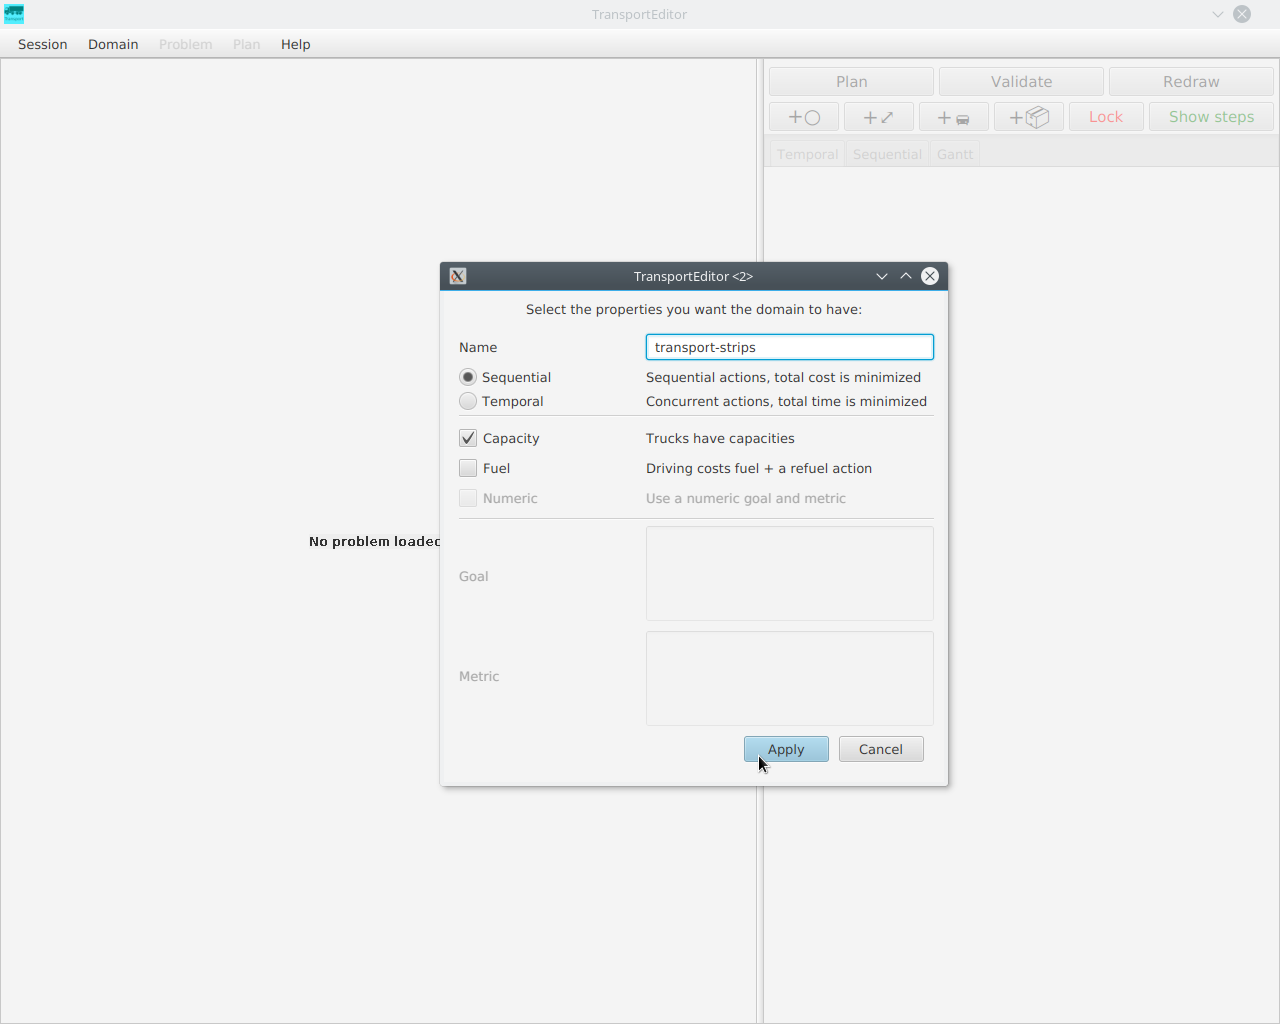
\includegraphics[width=0.91\textwidth]{../img/transporteditor_dom-creat}
Selecting a domain variant.
\end{center}
\medskip

\begin{center}
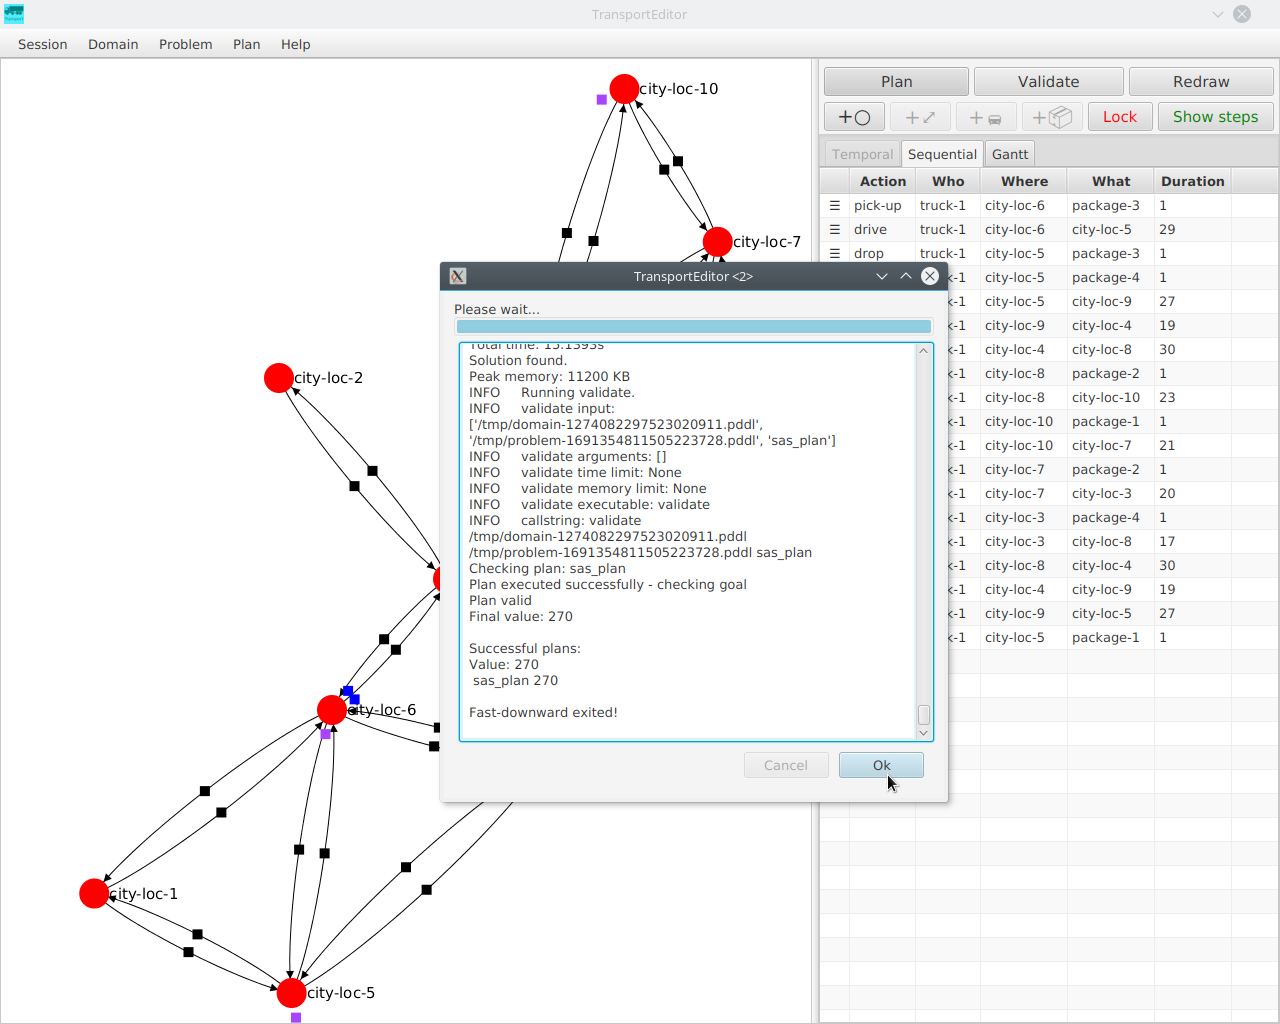
\includegraphics[width=0.91\textwidth]{../img/transporteditor_planning}
Running an external planner on a sequential problem.
\end{center}
\medskip

\begin{center}
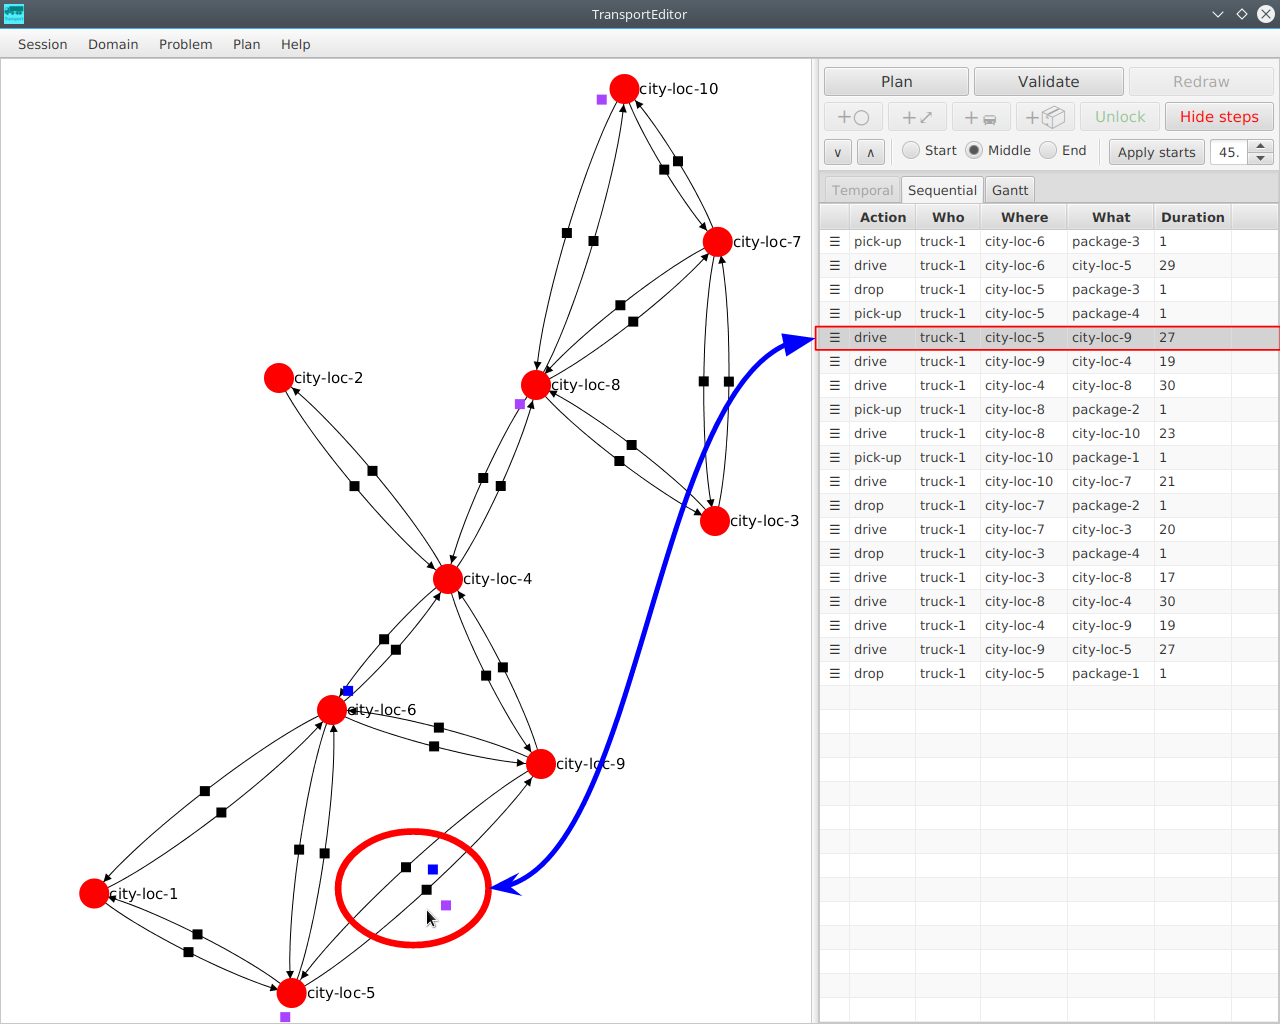
\includegraphics[width=0.94\textwidth]{../img/transporteditor_planstates}
Tracing a sequential plan. Highlighted is the corresponding \verb+drive+ action and the visualization of the vehicle (blue square) and the package it carries (purple square) on the road graph.
\end{center}
\medskip

\begin{center}
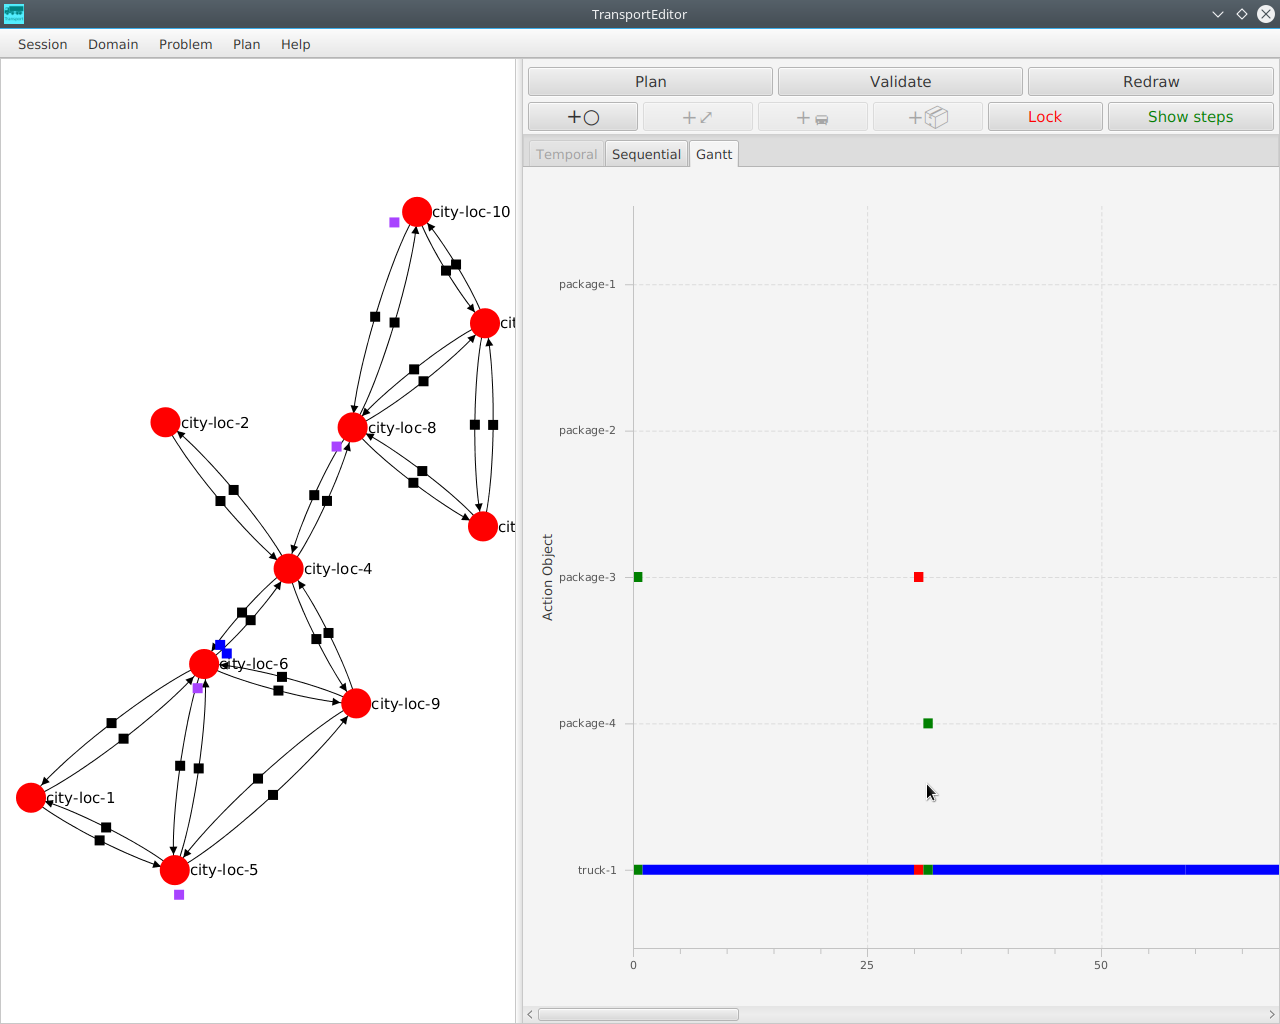
\includegraphics[width=0.94\textwidth]{../img/transporteditor_gantt}
Visualizing the plan as a Gantt chart.
\end{center}
